% This LaTeX was auto-generated from MATLAB code.
% To make changes, update the MATLAB code and export to LaTeX again.

\documentclass{article}

\usepackage[utf8]{inputenc}
\usepackage[T1]{fontenc}
\usepackage{lmodern}
\usepackage{graphicx}
\usepackage{color}
\usepackage{hyperref}
\usepackage{amsmath}
\usepackage{amsfonts}
\usepackage{epstopdf}
\usepackage[table]{xcolor}
\usepackage{matlab}

\sloppy
\epstopdfsetup{outdir=./}
\graphicspath{ {./random_distribution_images/} }

\begin{document}

\matlabtitle{Define distributions}

\begin{matlabcode}
mean = 50
\end{matlabcode}
\begin{matlaboutput}
mean = 50
\end{matlaboutput}
\begin{matlabcode}
uniform = randi([0 100],100000, 1);
gaussian = normrnd(mean,5,[100000 1]); 
\end{matlabcode}


\matlabheading{Rayleigh distribution:}

\begin{matlabcode}
alpha = mean/sqrt(pi/2)
\end{matlabcode}
\begin{matlaboutput}
alpha = 39.8942
\end{matlaboutput}
\begin{matlabcode}
vari = (2-pi/2)*alpha^2
\end{matlabcode}
\begin{matlaboutput}
vari = 683.0989
\end{matlaboutput}
\begin{matlabcode}
rayleigh = normrnd(mean, sqrt(vari), [100000 1]);
\end{matlabcode}


\begin{matlabcode}
histogram(gaussian)
\end{matlabcode}
\begin{center}
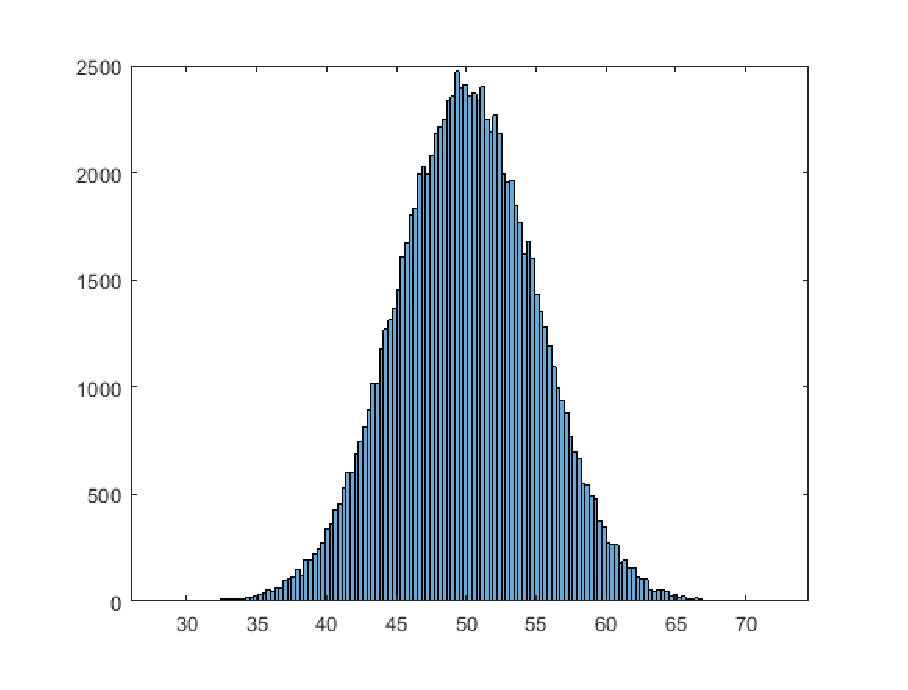
\includegraphics[width=\maxwidth{56.196688409433015em}]{figure_0.eps}
\end{center}
\begin{matlabcode}
histogram(uniform)
\end{matlabcode}
\begin{center}
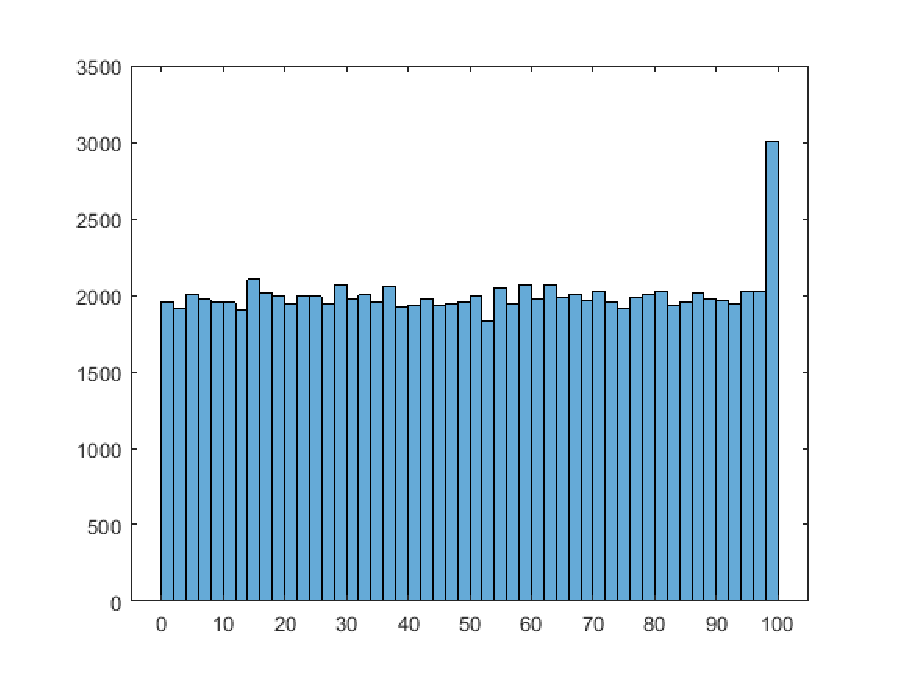
\includegraphics[width=\maxwidth{56.196688409433015em}]{figure_1.eps}
\end{center}
\begin{matlabcode}
histogram(rayleigh)
\end{matlabcode}
\begin{center}
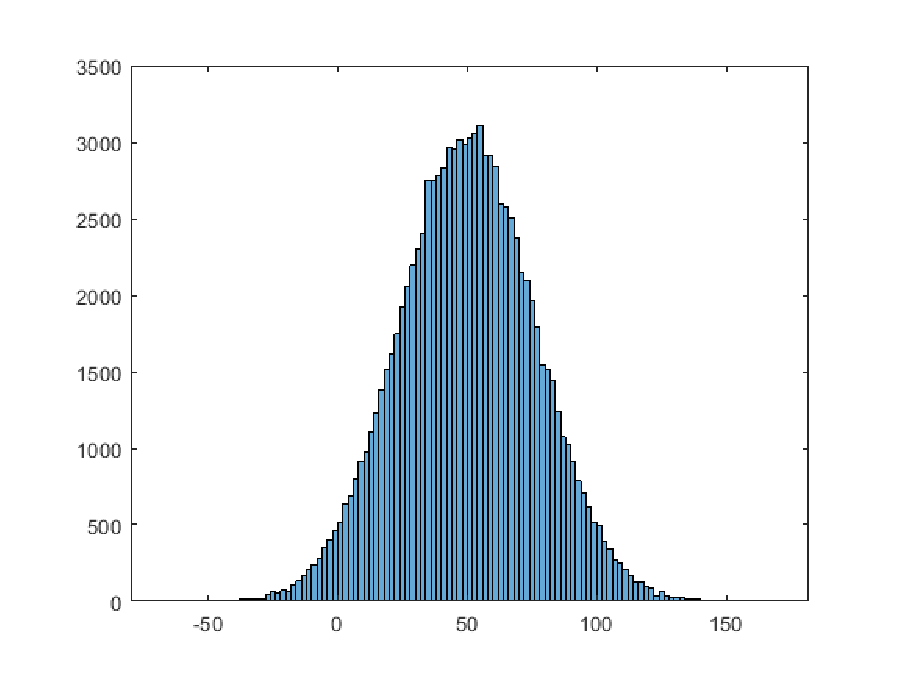
\includegraphics[width=\maxwidth{56.196688409433015em}]{figure_2.eps}
\end{center}


\matlabheading{Ideal Estimator Given no observation}

\begin{matlabcode}
x_prediction = mean % always predict mean a/c to l.m.s criterion
\end{matlabcode}
\begin{matlaboutput}
x_prediction = 50
\end{matlaboutput}
\begin{matlabcode}
% calculate error with all distribution: 
uniform_error = uniform - x_prediction;
gaussian_error = gaussian - x_prediction; 
rayleigh_error = rayleigh - x_prediction; 
c1_base = sum(uniform_error.^2)
\end{matlabcode}
\begin{matlaboutput}
c1_base = 85014905
\end{matlaboutput}
\begin{matlabcode}
c2_base = sum(gaussian_error.^2)
\end{matlabcode}
\begin{matlaboutput}
c2_base = 2.5003e+06
\end{matlaboutput}
\begin{matlabcode}
c3_base = sum(rayleigh_error.^2)
\end{matlabcode}
\begin{matlaboutput}
c3_base = 6.8434e+07
\end{matlaboutput}


\matlabheading{Change estimator to a random value and check if error decreases}

\begin{matlabcode}
x_prediction = randi([0, 100])
\end{matlabcode}
\begin{matlaboutput}
x_prediction = 73
\end{matlaboutput}
\begin{matlabcode}
% calculate error with all distribution: 
uniform_error = uniform - x_prediction;
gaussian_error = gaussian - x_prediction; 
rayleigh_error = rayleigh - x_prediction; 
c1 = sum(uniform_error.^2)
\end{matlabcode}
\begin{matlaboutput}
c1 = 137560199
\end{matlaboutput}
\begin{matlabcode}
c2 = sum(gaussian_error.^2)
\end{matlabcode}
\begin{matlaboutput}
c2 = 5.5385e+07
\end{matlaboutput}
\begin{matlabcode}
c3 = sum(rayleigh_error.^2)
\end{matlabcode}
\begin{matlaboutput}
c3 = 1.2099e+08
\end{matlaboutput}


\begin{matlabcode}

e_coefficient = [c1/c1_base c2/c2_base c3/c3_base].*100; 
e_coefficient+" % of c_1"
\end{matlabcode}
\begin{matlaboutput}
ans = 1x3 string    
"161.80715 % of c_1"    "2215.1746 % of c_1"    "176.80081 % of c_1"    

\end{matlaboutput}
\begin{matlabcode}
% since e_coefficient contains all percentages greater than 100, the l.m.s
% criterion provides a good estimator given no information about the
% distribution, with only mean and variance of the distribution known. 
\end{matlabcode}

\end{document}
